\documentclass[12pt,letterpaper,boxed,cm]{hmcpset}

\usepackage[margin=1in]{geometry}
\usepackage{mathtools}
\usepackage{mathrsfs}
\usepackage{graphicx}
\usepackage{cases}
\usepackage{braket}

\name{~}
\class{Physics 84}
\assignment{Homework 2}
\duedate{2/9/17}

\newcommand{\pn}[1]{\left( #1 \right)}
\newcommand{\abs}[1]{\left| #1 \right|}
\newcommand{\bk}[1]{\left[ #1 \right]}
\newcommand{\matelem}[3]{\big\langle #1\big\vert #2\big\vert #3\big\rangle}


\begin{document}
\problemlist{1, 2, 3, 4}

\begin{problem}[1.]
    \textbf{The 2-bit Deutsch-Jozsa algorithm}
     
    The $n$-bit Deutsch-Jozsa algorithm determines whether a two-valued function of an $n$-bit string, $f:\{0,1\}^{\otimes n} \rightarrow \{0,1\}$, is constant or balanced.  (For $n>1$ most functions are neither constant \textit{nor} balanced, but in this scenario we are assured that $f$ must be either one or the other; we only need to decide which.)  An oracle F takes an $n$-bit input $x$ (or $\ket{x}$) and a single target bit $y$ (or $\ket{y}$).  It computes $f(x)$ by taking $y$ to $y \oplus f(x)$ (or $\ket{y}$ to $\ket{y \oplus f(x)}$) just as in the one-bit algorithm.  In the quantum case, $\ket{x}$ is an $n$-qubit basis state; \textit{e.g.}, $\ket{0}\ket{1}\ket{0}\ket{0}...\ket{1}$ to represent $x=0100...1$.\\

    In the classical case, we call the oracle on different $x$ inputs and record all the $f(x)$ values.  We argued in class that the oracle must be called $2^{n-1}+1$ times in the worst-case scenario.  In this problem, you will show that a quantum circuit requires just one call to the oracle.   
    \begin{enumerate}
        \item [(a)]  Let $f$ be a constant or balanced function $f:\{0,1,2,3\} \rightarrow \{0,1\}$, or using binary notation for the input numbers, $f:\{00,01,10,11\} \rightarrow \{0,1\}$.  Explain, by determining the relevant properties of the 3-qubit state through the stages of the computation, what two-qubit measurement result you must get in the circuit below if the oracle encodes a constant $f$.
        \begin{center}
            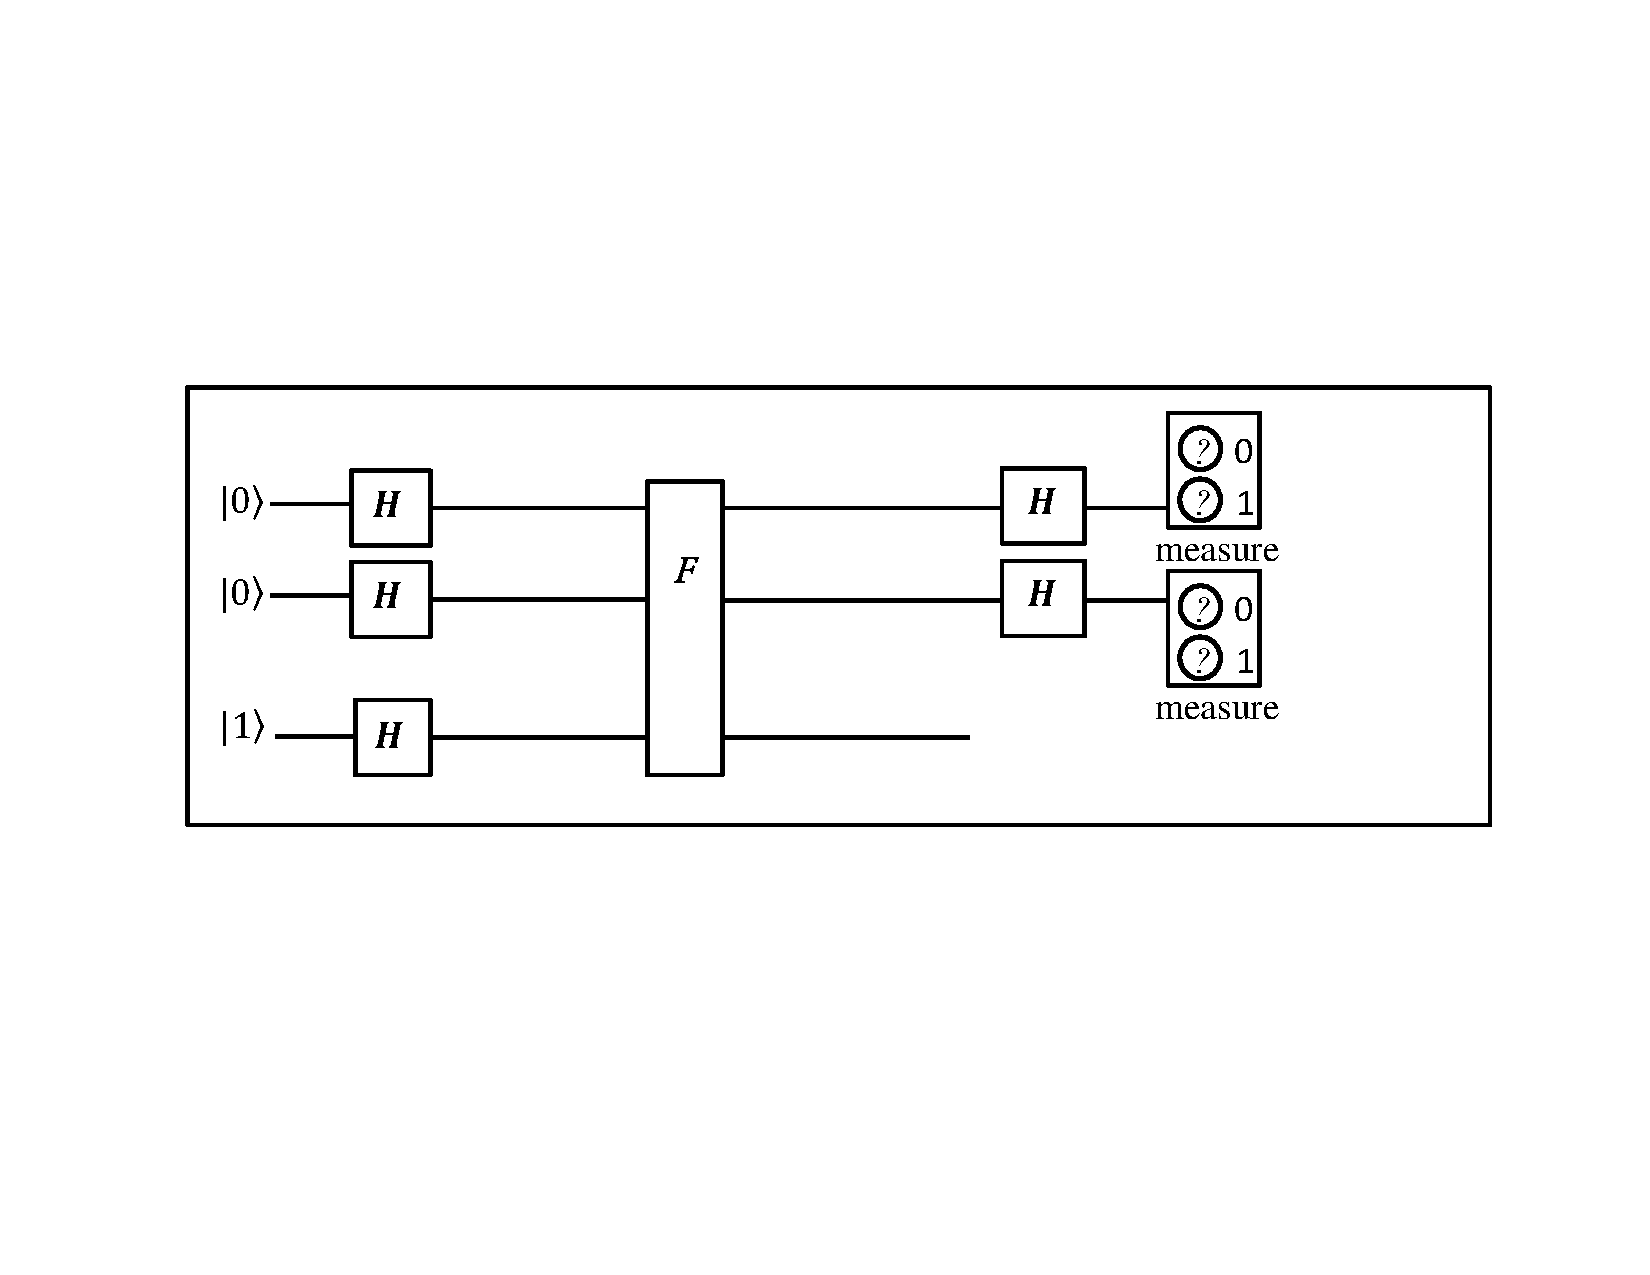
\includegraphics[width=280pt]{fig2-1-0.pdf}
        \end{center}
        \item [(b)] Consider the same circuit as in part (b), but let the oracle encode a balanced function $f$.  Show that you can \textit{never} get the same two-qubit measurement result as you were guaranteed in part (b).  [Hint:  Show that the state after the oracle F for a balanced function is orthogonal to the state after the oracle F for a constant function.  Unitary evolution preserves orthogonality, so now you know that the state right before measurement for a balanced function is orthogonal to the state right before measurement for a constant function.  Use that to show the measurement always yields different results for a balanced function vs. a constant one.]
    \end{enumerate}
\end{problem}

\begin{problem}[1. cont.]
    \begin{enumerate}
        \item [(c)] Now let $f$ be a constant or balanced function $f:\{0,1\}^{\otimes n} \rightarrow \{0,1\}$.  Explain, by determining the relevant properties of the $(n+1)$-qubit state through the stages of the computation, how the following quantum circuit solves the problem with a single call to the oracle.  This solution is the $n$-bit or generalized Deutsch-Jozsa algorithm; though David Deutsch and Richard Jozsa contributed greatly to its development, the algorithm in its present form was actually published by Richard Cleve, Artur Ekert, Chiara Macchiavello, and Michele Mosca in 1998. (See, \textit{e.g.}, arxiv.org/abs/quant-ph/9708016 after you have solved this homework problem.)
        \begin{center}
            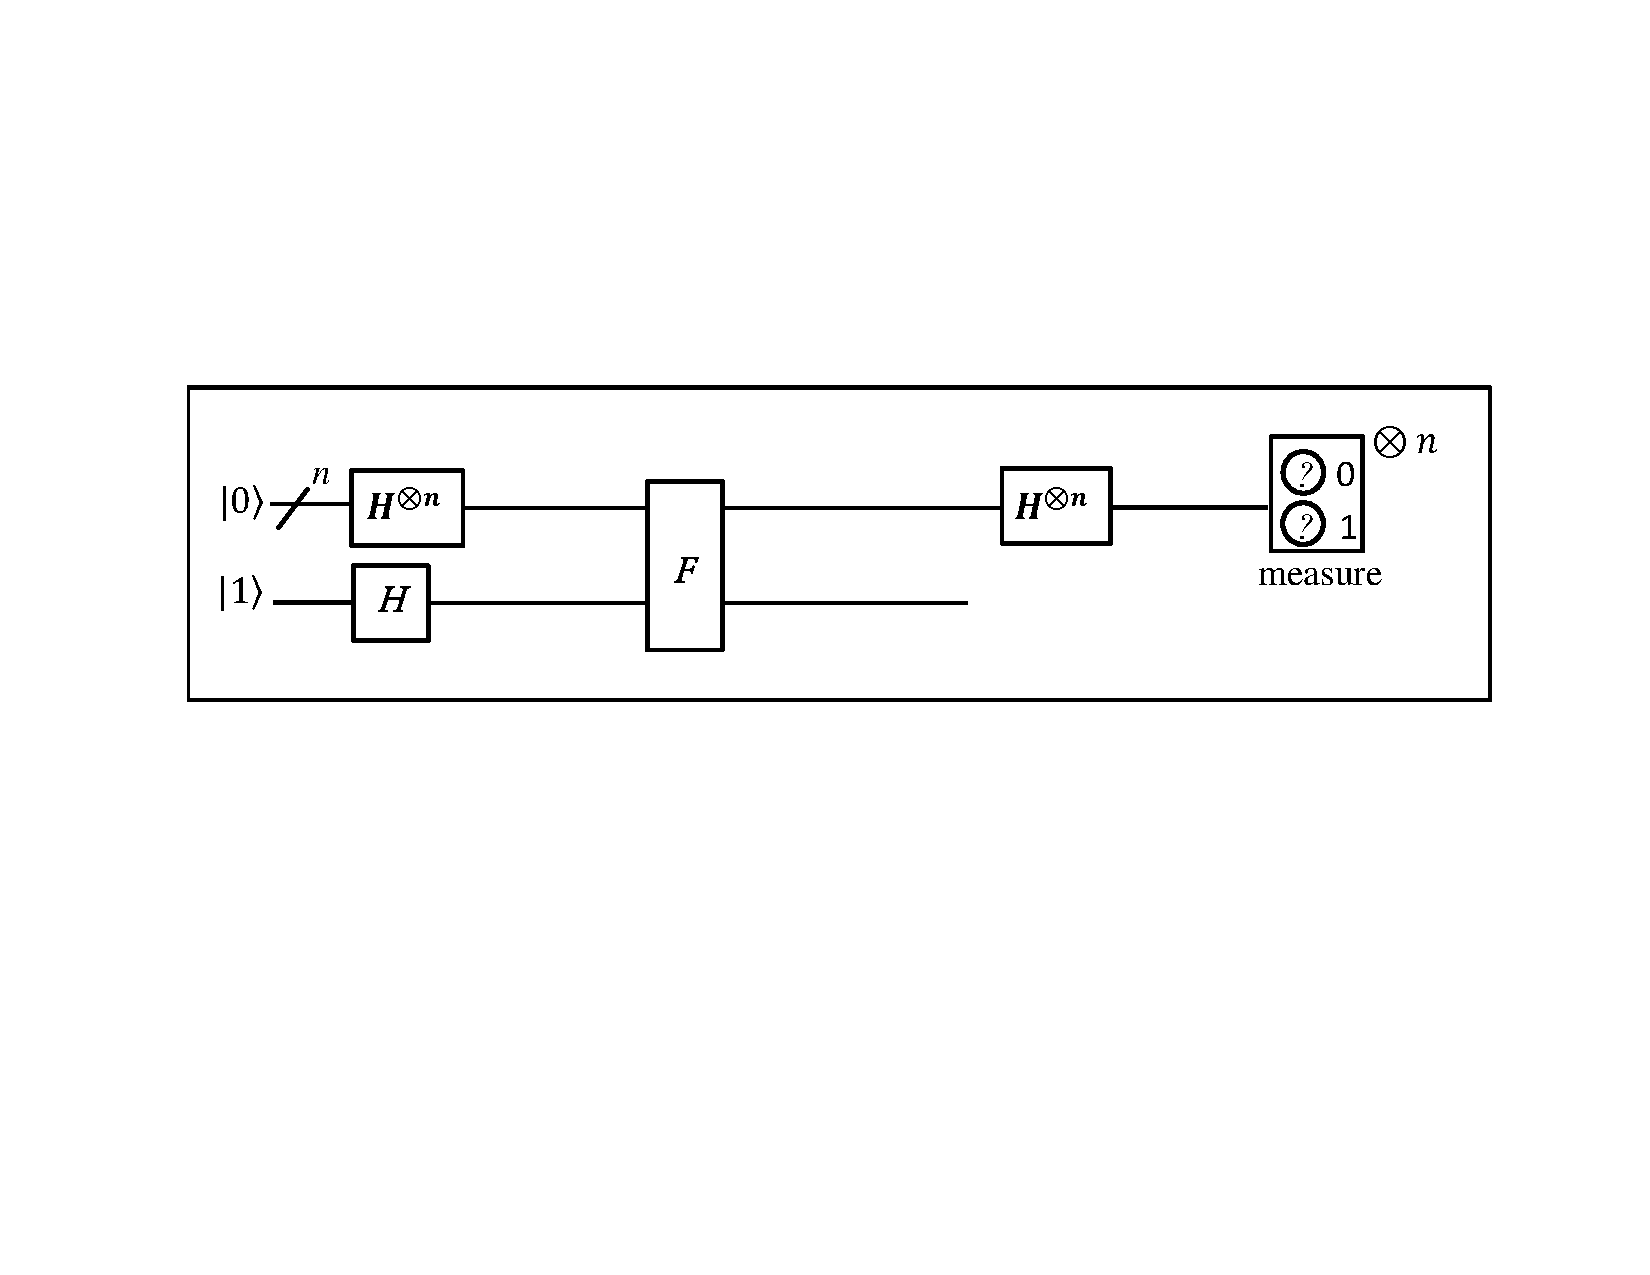
\includegraphics[width=300pt]{fig2-1-1.pdf} 
        \end{center}
    \end{enumerate}
\end{problem}

\begin{solution}
    \vfill
\end{solution}
\newpage

\begin{problem}[2.]
    \textbf{Creating entangled states}\\
    One of the entangled ``Bell states'' of two qubits is
    \[
        \ket{\Psi^-} = \frac{\ket{0}_A\ket{1}_B - \ket{1}_A\ket{0}_B}{\sqrt{2}}.
    \]
    Design a quantum logic circuit, using gates we have discussed in class, to create this two-qubit state starting from input qubits in the computational basis states $\ket{0}$ or $\ket{1}$.  Show that your circuit produces the state $\ket{\Psi^-}$ as its output.
\end{problem}

\begin{solution}
    \vfill
\end{solution}
\newpage

\begin{problem}[3.]
    \textbf{Measurements on one member of an entangled pair}\\
    Consider the two-qubit state $\ket{\Psi^-}$, but imagine that we perform a measurement on qubit $A$ only.
    \begin{enumerate}
        \item [(a)] Consider measuring qubit $A$ in the $\{\ket{0}_A,\ket{1}_A\}$ basis.  The probability of finding qubit $A$ in state $\ket{0}_A$ is given by
        \[
            \matelem{\Psi^-}{\hat{P}_{0,A} \otimes \hat{I}_B}{\Psi^-};
        \]
        here, the single-qubit projection operator $\hat{P}_{0}$ acting on qubit $A$ is tensored with the identity operator $\hat{I}$ acting on qubit $B$ since no measurement is performed on qubit $B$. Show that the probability of finding qubit $A$ in state $\ket{0}_A$ is $1/2$.
        \item [(b)] We may choose to write each qubit's state, not as a superposition of $\ket{0}$ and $\ket{1}$, but as a superposition of $\ket{\psi}$ and $\ket{\psi_\perp}$, where $\ket{0} = \alpha\ket{\psi} + \beta\ket{\psi_\perp}$, $\ket{1} = -\beta^*\ket{\psi} +\alpha^*\ket{\psi_\perp}$, and $\abs{\alpha}^2+\abs{\beta}^2 = 1$.  Show that:
        \[
            \ket{\Psi^-} = \frac{\ket{\psi}_A\ket{\psi_\perp}_B - \ket{\psi_\perp}_A\ket{\psi}_B}{\sqrt{2}}.
        \]
        \item [(c)] If we measure qubit $A$ in \textit{any} $\{\ket{\psi}_A,\ket{\psi_\perp}_A\}$ basis, show that the probability of finding qubit $A$ in the state $\ket{\psi}_A$ is $1/2$.  Thus the state of qubit $A$ by itself, independent of the state of qubit $B$, is completely uncertain and contains no information.  This is the hallmark of complete entanglement between two particles. 
    \end{enumerate}
\end{problem}

\begin{solution}
    
\end{solution}
\newpage

\begin{problem}[4.]
    \textbf{Controlled U from CNOT and single-qubit unitaries}\\
    In class, we constructed a general two-qubit controlled $U$ gate from CNOT and single-qubit unitaries by first writing $U$ as $U=e^{i\alpha}AXBXC$.  Here $X = \begin{bmatrix} 0 & 1 \\ 1 & 0 \end{bmatrix}$ and $A$, $B$, and $C$ are unitary matrices such that $ABC=I$.
    \begin{enumerate}
        \item [(a)] Show that $XR_y\bigl(\Delta\bigr)X = R_y\bigl(-\Delta\bigr)$, where $R_y\bigl(\Delta\bigr) = \begin{bmatrix} \cos \frac{\Delta}{2} & -\sin \frac{\Delta}{2} \\ \sin \frac{\Delta}{2} & \cos \frac{\Delta}{2} \end{bmatrix}$ represents rotation by angle $\Delta$ about the $y$ axis on the Bloch sphere.
        \item [(b)] Show that $XR_z\bigl(\gamma\bigr)X = R_z\bigl(-\gamma\bigr)$, where $R_z\bigl(\gamma\bigr) = \begin{bmatrix} e^{-i\frac{\gamma}{2}} & 0 \\ 0 & e^{i\frac{\gamma}{2}} \end{bmatrix}$ represents rotation by angle $\gamma$ about the $z$ axis on the Bloch sphere.
        \item [(c)] Show that 
        \begin{align}
            A &= R_z\bigl(\beta'\bigr) R_y\bigl(\frac{\Delta}{2}\bigr) \nonumber \\
            B &= R_y\bigl(-\frac{\Delta}{2}\bigr)R_z\bigl(-\frac{(\beta+\beta')}{2}\bigr) \nonumber \\
            C &= R_z\bigl(\frac{\beta-\beta'}{2}\bigr) \nonumber
        \end{align}
        satisfy the conditions set out above for expressing an arbitrary U.  That is, show that $ABC=I$ and that $e^{i\alpha}AXBXC$ gives a form we discussed in class for a general 2x2 unitary matrix.
    \end{enumerate}
\end{problem}

\begin{solution}
    \vfill
\end{solution}
\newpage
\end{document}